\documentclass{article}
\usepackage{lipsum}
\usepackage{braket}
\usepackage{mathrsfs}
\usepackage{amsmath}
\usepackage{graphicx}
\begin{document}
\title{Assignment 1}
\author{
    Name:\underline{Wang Dingrui}
}
\maketitle
\section*{EXERCISE 1: COMPLEX NUMBERS}
\begin{enumerate}
    \item Assume $x=a_1+b_1i$, $x=a_2+b_2i$, $x=a_3+b_3i$,

          we have $x+y+z=a_1+a_2+a_3+(b_1+b_2+b_3)i$,

          To a complex number $n=a+bi$ we have $n^*=a-bi$,

          so

          $|x|^2=x\cdot x^*=a_1^2-b_1^2(i)^2=a_1^2-b_1^2\cdot(-1)=a_1^2+b_1^2$,

          $x^*y \\= (a_1-b_1i)\cdot(a_2+b_2i)\\=a_1a_2+a_1b_2i-a_2b_1i-b_1b_2i^2\\=a_1a_2+b_1b_2+(a_1b_2-a_2b_1)i$,

          $Re(x^*y)=a_1a_2+b_1b_2$,

          similarly, we have

          $|y|^2=a_2^2+b_2^2$,

          $|z|^2=a_3^2+b_3^2$,

          $Re(y^*z)=a_2a_3+b_2b_3$

          $Re(x^*z)=a_1a_3+b_1b_3$

          and



          $(x+y+z)^*=a_1+a_2+a_3-(b_1+b_2+b_3)i$,

          $|x+y+z|^2\\=(x+y+z)\cdot(x+y+z)^*
              \\=((a_1+a_2+a_3)+(b_1+b_2+b_3)i)\cdot((a_1+a_2+a_3)-(b_1+b_2+b_3)i)
              \\=((a_1+a_2+a_3)^2-(b_1+b_2+b_3)^2\cdot(-1))
              \\=((a_1+a_2+a_3)^2+(b_1+b_2+b_3)^2)
              \\=a_1^2+a_2^2+a_3^2+2a_1a_2+2a_1a_3+2a_2a_3+b_1^2+b_2^2+b_3^2+2b_1b_2+2b_1b_3+2b_2b_3
              \\=a_1^2+b_1^2+a_2^2+b_2^2+a_3^2+b_3^2+2(a_1a_2+b_1b_2+a_2a_3+b_2b_3+a_1a_3+b_1b_3)
              \\=|x|^2+|y|^2+|z|^2+2[Re(x^*y)+Re(y^*z)+Re(x^*z)]
          $

          This shows that

          $|x+y+z|^2=|x|^2+|y|^2+|z|^2+2[Re(x^*y)+Re(y^*z)+Re(x^*z)]$
    \item $(i+2)(3-4i)/(2-i)
              \\=(3i-4i^2+2*3-2*4i)/(2-i)
              \\=(3i-4\times(-1)+2*3-2*4i)/(2-i)
              \\=(3i+4+6-8i)/(2-i)
              \\=(10-5i)/(2-i)
              \\=5(2-i)/(2-i)
              \\=5
          $
    \item $ (i-4)/(2i-3)
              \\=[(i-4)(2i+3)]/[(2i-3)(2i+3)]
              \\=(2i^2+3i-8i-4*3)/((2i)^2-3*3)
              \\=[2\times(-1)+3i-8i-4*3]/[4\times(-1)-3*3]
              \\=(-2-5i-12)/(-4-9)
              \\=(-14-5i)/(-13)
              \\=[(-1)(14+5i)]/(-1\times13)
              \\=(14+5i)/13
              \\=14/13+(5/13)i
          $

          so, the real part is $14/13$ and imaginary pary is $5/13$.
    \item $i^{33}
              \\=i^{32}i
              \\=i^{2\times16}i
              \\=(i^2)^{16}i
              \\=(-1)^{16}i
              \\=i
          $

          so, the absolute value of $i^{33}$ is $|i|$

          $|i| = |0+i| = \sqrt{|0+i|^2} = \sqrt{(0+i)(0+i)^*}=\sqrt{(0+i)(0-i)}=\sqrt{-i^2}=\sqrt{-(-1)}=\sqrt{1}=1$
    \item \begin{enumerate}
              \item[i.] For complex number $c_1=a_1+b_1i$ and $c_2=a_2+b_2i$, we have
                    \[|c_1|^2=a_1^2+b_1^2\]
                    \[|c_2|^2=a_2^2+b_2^2\]
                    \[|c_1+c_2|^2=(a_1+a_2)^2+(b_1+b_2)^2
                        \\=a_1^2+a_2^2+2a_1a_2+b_1^2+b_2^2+2b_1b_2\]

                    so we need to find $a_1,a_2,b_1,b_2$ that makes
                    \[a_1^2+a_2^2+2a_1a_2+b_1^2+b_2^2+2b_1b_2\geq a_1^2+b_1^2\]
                    and
                    \[a_1^2+a_2^2+2a_1a_2+b_1^2+b_2^2+2b_1b_2<a_2^2+b_2^2\]
                    so we have
                    \[a_2^2+2a_1a_2+b_2^2+2b_1b_2\geq 0\]
                    and
                    \[a_1^2+2a_1a_2+b_1^2+2b_1b_2<0\]
                    so, we need $2a_1a_2+2b_1b_2\geq-(a_2^2+b_2^2)$ and $2a_1a_2+2b_1b_2<-(a_1^2+b_1^2)$,

                    which means $-(a_2^2+b_2^2)\leq 2a_1a_2+2b_1b_2<-(a_1^2+b_1^2)$,

                    Through observing, it is easy to find $a_1=-1,a_2=3,b_1=1,b_2=-3$ makes $|c_1+c_2|^2\geq |c_1|^2$ and $|c_1+c_2|^2< |c_2|^2$.

              \item[ii.]
                    Yes. For $c_1=-1+2i,c_2=2-i$, $c_1+c_2=1+i$

                    $|c_1+c_2|^2==2$

                    $|c_1|^2=5$

                    $|c_2|^2=5$

                    in this case, two complex numbers satisfy $|c_1 + c_2|^2\leq|c_1|^2$ and $|c_1 + c_2|^2\leq|c_2|^2$.

          \end{enumerate}
    \item Assume both $\vec{v}_1$ and $\vec{v}_2$ has a length of $n$.

          $\vec{v}_1=(\psi_{10},\psi_{11},\psi_{12},\psi_{13},...,\psi_{1n})^T$,

          $\vec{v}_2=(\psi_{20},\psi_{21},\psi_{22},\psi_{23},...,\psi_{2n})^T$.

          For real vectors $\vec{r}_1$ and $\vec{r}_2$, we have $\langle \vec{r}_1,\vec{r}_2 \rangle=\vec{r}_1^T\vec{r}_2$.

          Similarly, we can define the inner product of $\vec{v}_1,\vec{v}_2$ that
          \[\langle \vec{v}_1,\vec{v}_2 \rangle
              \\=\vec{v}_1^T\vec{v}_2
          \]
          where $\vec{v}_1^T$ is the transpose of $\vec{v}_1$.

          This means
          \[
              \langle \vec{v}_1,\vec{v}_2 \rangle=\\=(\psi_{10}^*,\psi_{11}^*,\psi_{12}^*,\psi_{13}^*,...,\psi_{1n}^*)(\psi_{20},\psi_{21},\psi_{22},\psi_{23},...,\psi_{2n})^T
          \]
          so,
          \[\langle \vec{v}_1,\vec{v}_2 \rangle=\sum_{i=0}^{n-1}\psi_{1i}\psi_{2i}\]
          The properties of an inner product $\langle,\rangle$ are as followed\cite{ref1}.
          \begin{enumerate}
              \item \textbf{Linearity:} $\langle a\mathbf{u}+b\mathbf{v},\mathbf{w}\rangle=a\langle \mathbf{u,w}\rangle+b\langle \mathbf{v,w}\rangle$
              \item \textbf{Symmetric Property: }$\langle \mathbf{u,v}\rangle=\langle \mathbf{v,u}\rangle$ (For  complex vectors, the inner product doesn't satisfy this property.)
              \item \textbf{Positive Definite Property: } For any $\mathbf{u\in V}$, $\langle \mathbf{u,u}\rangle\geq0$;
                    and $\langle \mathbf{u,u}\rangle=0$ if and only if $\mathbf{u}=0$;
          \end{enumerate}
          For complex vectors $\vec{v1},\vec{v_2},\vec{v_3}$, all of them have a length of n.

          $\langle a\vec{v_1}+b\vec{v_2},\vec{v_3}\rangle
              \\=\sum_{i=0}^{n-1}(a\psi_{1i}^*+b\psi_{2i}^*)(\psi_{3i})
              \\=\sum_{i=0}^{n-1}(a\psi_{1i}^*)(\psi_{3i})+\sum_{i=0}^{n-1}(b\psi_{2i}^*)(\psi_{3i})
              \\=a\sum_{i=0}^{n-1}(\psi_{1i}^*)(\psi_{3i})+b\sum_{i=0}^{n-1}(\psi_{2i}^*)(\psi_{3i})
              \\=a\langle\vec{v_1},\vec{v_3}\rangle+b\langle\vec{v_2},\vec{v_3}\rangle
          $

          This proves the linearity.

          Also, we have

          $\langle \vec{v_1},\vec{v_2}\rangle
              \\=\sum_{i=0}^{n-1}\psi_{1i}^*\psi_{2i}$

          $
          \langle\vec{v_2},\vec{v_1}\rangle
              \\=\sum_{i=0}^{n-1}\psi_{2i}^*\psi_{1i}
          $

          Because $\sum_{i=0}^{n-1}\psi_{1i}^*\psi_{2i}$ doesn't equal to $\sum_{i=0}^{n-1}\psi_{2i}^*\psi_{1i}$, the inner product of complex numbers doesn't have the symmetric property.

          For any complex vector $\vec{v_1}$, $\langle \vec{v_1},\vec{v_1}\rangle=\sum_{i=0}^{n-1}\psi_{1i}^*\psi_{1i}=\sum_{i=0}^{n-1}|\psi_{1i}|^2$.
          For any complex number $\psi=a+bi$, we have $|\psi|^2=a^2+b^2\geq0$,

          so $\langle \vec{v_1},\vec{v_1}\rangle=\sum_{i=0}^{n-1}|\psi_{1i}|^2\geq0$ and $\vec{v_1}$ is a complex vector, so $|\vec{v_1}|\neq0$.

          This proves the positive definite property.

          So, it satisfies the properties of Linearity and Positive Definite of an inner product, but doesn't satisfy a property of Symmetric.
\end{enumerate}
\section*{EXERCISE 2: THE TENSOR PRODUCT}
\begin{enumerate}
    \item
          $\ket{0}_A\otimes\ket{1}_B
              \\=\left(\begin{array}{c}1\\0\end{array}\right)\otimes\left(\begin{array}{c}0\\1\end{array}\right)
              \\=\left(\begin{array}{c}1\cdot{\left(\begin{array}{c}0\\1\end{array}\right)}\\0\cdot{\left(\begin{array}{c}0\\1\end{array}\right)}\end{array}\right)
              \\=\left(\begin{array}{c}1\times0\\1\times1\\0\times0\\0\times1\end{array}\right)
              \\=\left(\begin{array}{c}0\\1\\0\\0\end{array}\right)
              \\=0(\ket{0}\otimes\ket{0})+1(\ket{0}\otimes\ket{1})+0(\ket{1}\otimes\ket{0})+0(\ket{1}\otimes\ket{1})
          $
    \item
          $\ket{+}_A\otimes\ket{-}_B
              \\=\left(\begin{array}{c}\frac{1}{\sqrt{2}}\\\frac{1}{\sqrt{2}}\end{array}\right)\otimes\left(\begin{array}{c}\frac{1}{\sqrt{2}}\\-\frac{1}{\sqrt{2}}\end{array}\right)
              \\=\left(\begin{array}{c}\frac{1}{\sqrt{2}}\cdot{\left(\begin{array}{c}\frac{1}{\sqrt{2}}\\-\frac{1}{\sqrt{2}}\end{array}\right)}\\\frac{1}{\sqrt{2}}\cdot{\left(\begin{array}{c}\frac{1}{\sqrt{2}}\\-\frac{1}{\sqrt{2}}\end{array}\right)}\end{array}\right)
              \\=\left(\begin{array}{c}\frac{1}{\sqrt{2}}\times\frac{1}{\sqrt{2}}\\\frac{1}{\sqrt{2}}\times-\frac{1}{\sqrt{2}}\\\frac{1}{\sqrt{2}}\times\frac{1}{\sqrt{2}}\\\frac{1}{\sqrt{2}}\times-\frac{1}{\sqrt{2}}\end{array}\right)
              \\=\left(\begin{array}{c}\frac{1}{2}\\-\frac{1}{2}\\\frac{1}{2}\\-\frac{1}{2}\end{array}\right)
              \\=\frac{1}{2}(\ket{0}\otimes\ket{0})-\frac{1}{2}(\ket{0}\otimes\ket{1})+\frac{1}{2}(\ket{1}\otimes\ket{0})-\frac{1}{2}(\ket{1}\otimes\ket{1})
          $
    \item
          $\ket{0}_A\otimes\ket{-}_B
              \\=\frac{1}{\sqrt{2}}(\ket{+}+\ket{-})\otimes\ket{-}
              \\=\frac{1}{\sqrt{2}}\ket{+}\otimes\ket{-}+\frac{1}{\sqrt{2}}\ket{-}\otimes\ket{-}
              \\=0\times\ket{+}\otimes\ket{+}+\frac{1}{\sqrt{2}}\ket{+}\otimes\ket{-}+0\times\ket{-}\otimes\ket{+}+\frac{1}{\sqrt{2}}\ket{-}\otimes\ket{-}
          $
    \item $\ket{1}_A\otimes\ket{1}_B
              \\=\frac{1}{\sqrt{2}}(\ket{+}-\ket{-})\otimes\frac{1}{\sqrt{2}}(\ket{+}-\ket{-})
              \\=\frac{1}{2}(\ket{+}\otimes\ket{+})-\frac{1}{2}(\ket{+}\otimes\ket{-})-\frac{1}{2}(\ket{-}\otimes\ket{+})+\frac{1}{2}(\ket{-}\otimes\ket{-})
          $
    \item We have
          $\ket{\Phi^+}
              \\=\frac{1}{\sqrt{2}}(\ket{0}_A\otimes\ket{1}_B+\ket{1}_A\otimes\ket{0}_B)
              \\=\frac{1}{\sqrt{2}}(\left(\begin{array}{c}1\\0\end{array}\right)\otimes\left(\begin{array}{c}0\\1\end{array}\right)+\left(\begin{array}{c}0\\1\end{array}\right)\otimes\left(\begin{array}{c}1\\0\end{array}\right))
              \\=\frac{1}{\sqrt{2}}(\left(\begin{array}{c}0\\1\\0\\0\end{array}\right)+\left(\begin{array}{c}0\\0\\1\\0\end{array}\right))
              \\=\frac{1}{\sqrt{2}}(\left(\begin{array}{c}0\\1\\1\\0\end{array}\right))
          $

          For $A=\left(\begin{array}{c}
                      a_0 \\a_1
                  \end{array}\right)$ and $B=\left(\begin{array}{c}
                      b_0 \\b_1
                  \end{array}\right)$,
          we have $A\otimes B=\left(\begin{array}{c}
                      a_0b_0 \\a_0b_1\\a_1b_0\\a_1b_1
                  \end{array}\right)$.

          If $\ket{\Phi^+}$ can be written as $A\otimes B$, then

          $a_0b_0=0\\a_0b_1=\frac{1}{\sqrt{2}}\\a_1b_0=\frac{1}{\sqrt{2}}\\a_1b_1=0$.

          To make $a_0b_0=0$, either $a_0=0$ or $b_0=0$ should be true.

          If any of them is true, then $a_0b_1=\frac{1}{\sqrt{2}}$ and $a_1b_0=\frac{1}{\sqrt{2}}$ cannot be true in the same time.

          So $\ket{\Phi^+}$ can not be written as $A\otimes B$.
    \item We have $\ket{0}\ket{0}=\left(\begin{array}{c}
                      1 \\0\\0\\0
                  \end{array}\right)$ and $\ket{1}\ket{1}=\left(\begin{array}{c}
                      0 \\0\\0\\1
                  \end{array}\right)$.

          We also have
          $\ket{+}\ket{-}=\frac{1}{2}(\ket{0}\ket{0}-\ket{1}\ket{1})$

          and $\ket{-}\ket{+}=\frac{1}{2}(\ket{0}\ket{0}-\ket{1}\ket{1})$

          $\ket{\Phi^-}=\frac{1}{\sqrt{2}}(\ket{0}_A\otimes\ket{1}_B-\ket{1}_A\otimes\ket{0}_B)$

          So, $-\ket{\Phi^-}
              \\=\frac{1}{\sqrt{2}}(\ket{1}_A\otimes\ket{0}_B-\ket{0}_A\otimes\ket{1}_B)
              \\=\frac{1}{\sqrt{2}}(\left(\begin{array}{c}
                      0 \\0\\0\\0
                  \end{array}\right)-\left(\begin{array}{c}
                      0 \\0\\0\\0
                  \end{array}\right))
              \\=\left(\begin{array}{c}
                      0 \\0\\0\\0
                  \end{array}\right)
              \\=\frac{1}{\sqrt{2}}[\frac{1}{2}(\ket{0}\ket{0}-\ket{1}\ket{1})-\frac{1}{2}(\ket{0}\ket{0}-\ket{1}\ket{1})]
              \\=\frac{1}{\sqrt{2}}(\ket{+}\ket{-}-\ket{-}\ket{+})
              % \\=\frac{1}{\sqrt{2}}[(\left(\begin{array}{c}
              %     1\\0\\0\\0
              % \end{array}\right)-\left(\begin{array}{c}
              %     0\\0\\0\\1
              % \end{array}\right))-(\left(\begin{array}{c}
              %     1\\0\\0\\0
              % \end{array}\right)-\left(\begin{array}{c}
              %     0\\0\\0\\1
              % \end{array}\right))]
              % \\==\frac{1}{\sqrt{2}}\times2\times(\ket{0}\ket{0}-\ket{1}\ket{1})
              % \\=\frac{2}{\sqrt{2}}[(\ket{0}+\ket{1})\otimes(\ket{0}-\ket{1})]
              % \\=
          $

          So $\ket{\Phi^-}$ in basis $\mathcal{B}_1$ is equal to $-\ket{\Phi^-}$ in basis $\mathcal{B}_2$.

\end{enumerate}
\section*{OVERLAPS OF STATES}
\begin{enumerate}
    \item For $\ket{\psi}=\left(\begin{array}{c}
                      c_0 \\c_1\\...\\c_{n-1}
                  \end{array}\right)$
          where $c_k=a_k+b_ki$,
          we know

          $\lVert\psi\rVert^2_2 = \sum_{i=0}^{n-1}|c_i|^2=\sum_{i=0}^{n-1}a_i^2+b_i^2$.

          now,


          $\braket{\psi|\psi}
              \\=\left(c_0^*,c_1^*,...,c_{n-1}^*\right)\left(\begin{array}{c}
                      c_0 \\c_1\\...\\c_{n-1}
                  \end{array}\right)
              \\=\sum_{i=0}^{n-1}c_i^*c_imaginary
              \\=\sum_{i=0}^{n-1}a_i^2+b_i^2
              \\=\lVert\psi\rVert^2_2
          $

          So, $\braket{\psi|\psi}=\lVert\psi\rVert^2_2$
    \item
          \begin{enumerate}
              \item For $\ket{\psi_1}=\frac{1}{3}\ket{-}$,

                    $\lVert\psi_1\rVert^2
                        \\=\braket{\psi_1|\psi_1}
                        \\=\frac{1}{9}\braket{-|-}
                        \\=\frac{1}{9}[\frac{1}{2}\braket{0|0}+(-1)^2\frac{1}{2}\braket{1|1}]
                        \\=\frac{1}{9}(\frac{1}{2}+\frac{1}{2})
                        \\=\frac{1}{9}$

                    so,

                    $\lVert\psi_1\rVert=\sqrt{\lVert\psi_1\rVert^2}=\sqrt{\frac{1}{9}}=\frac{1}{3}$

              \item For $\ket{\psi_2}=\frac{1}{\sqrt{2}}(i\ket{0}+\ket{1})$

                    $\lVert\psi_2\rVert^2
                        \\=\frac{1}{2}\times -(i^2\times\braket{0|0})+\frac{1}{2}\braket{1|1}
                        \\=\frac{1}{2}*1+\frac{1}{2}*1
                        \\=1
                    $

                    So, $\lVert\psi_2\rVert=\sqrt{1}=1$
              \item $\lVert\frac{2}{5}\ket{0}+\frac{3}{5}\ket{1}\rVert
                        \\=\sqrt{\frac{2}{5}\times\frac{2}{5}\braket{0|1}+\frac{2}{5}\times\frac{3}{5}\braket{0|0}+\frac{2}{5}\times\frac{3}{5}\braket{1|1}+\frac{3}{5}\times\frac{3}{5}\braket{1|1}}
                        \\=\sqrt{\frac{4}{25}\times1+\frac{9}{25}\times1}
                        \\=\sqrt{\frac{13}{25}}
                        \\=\frac{\sqrt{13}}{5}
                    $
          \end{enumerate}
    \item $\ket{\psi_2}=\frac{1}{\sqrt{2}}(i\ket{0}+\ket{1})$ is the correct normalization.

          The renormalized state $\ket{\psi_1}'=\frac{\ket{\psi_1}}{\frac{1}{3}}=\ket{-}$

          The renormalized state $\ket{\psi_3}'=\frac{\ket{\psi_3}}{\frac{\sqrt{13}}{5}}=\frac{2}{\sqrt{13}}\ket{0}+\frac{3}{\sqrt{13}}\ket{1}$
    \item State $\psi=\frac{1}{\sqrt{2}}\ket{0}+\frac{1}{\sqrt{2}}\ket{1}$.

          The probability $p_1$ to find $\ket{\psi}$ in state $\ket{1}$ is:
          \[p_1=|\braket{1|\psi}|^2=|(\frac{1}{\sqrt{2}})\braket{1|1}|^2=\frac{1}{2}\]


          The probability $p_2$ to find $\ket{\psi}$ in state $\ket{-}$ is:
          \[p_2=|\braket{-|\psi}|^2=|\braket{-|+}|^2=|\frac{1}{2}(\braket{0|0}-\braket{1|1})|^2=0\]

    \item The probability $p$ to find $\ket{\psi}=\frac{1}{\sqrt{2}}(i\ket{0}-\ket{1})$ in state $\ket{+}$ is:

          $p=|\braket{+|\psi}|^2=|\frac{1}{2}(i\braket{0|0}-\braket{1|1})|^2=\frac{1}{4}|-1+i|^2=\frac{1}{4}(1+1)=\frac{1}{2}$

    \item The probability $p$ of output $\ket{\psi}$ in the state $\ket{+}$ is:

          $p=|\braket{\phi|\psi}|^2=|[\frac{1}{\sqrt{2}}(\bra{0}+\bra{1})](\frac{2}{\sqrt{5}}\ket{0}+i\frac{1}{\sqrt{5}}\ket{1})|^2
              \\=|\frac{2}{\sqrt{10}}\braket{0|0}+0+0+i\frac{1}{\sqrt{10}}\braket{1|1}|^2
              \\=|\frac{2}{\sqrt{10}}+i\frac{1}{\sqrt{10}}|^2
              \\=\frac{4}{10}+\frac{1}{10}
              \\=\frac{1}{2}$

          $\frac{1}{2}=50\%>45\%$

          So, we accept this state.

\end{enumerate}
\section*{DENSITY OPERATORS}
\begin{enumerate}
    \item For $\ket{\psi}=\ket{+}_A\otimes\ket{0}$
          The density operator is $\ket{\psi}\bra{\psi}$

          $\ket{+}_A\otimes\ket{0}=\frac{1}{\sqrt{2}}(\ket{0}+\ket{1})\otimes\ket{0}=\frac{1}{\sqrt{2}}(\ket{0}\otimes\ket{0}+\ket{1}\otimes\ket{0})
              \\=\frac{1}{\sqrt{2}}(\left(\begin{array}{c}
                      1 \\0\\0\\0
                  \end{array}\right)+\left(\begin{array}{c}
                      0 \\0\\1\\0
                  \end{array}\right))
              \\==\frac{1}{\sqrt{2}}(\left(\begin{array}{c}
                      1 \\0\\1\\0
                  \end{array}\right))
          $

          The density matrix

          $\rho
              \\=\ket{+}_A\otimes\ket{0}_B\bra{+}_A\otimes\bra{0}_B
              \\=\frac{1}{2}\left(\begin{array}{c}
                      1 \\0\\1\\0
                  \end{array}\right)\left(\begin{array}{cccc}
                      1 & 0 & 1 & 0
                  \end{array}\right)
              \\=\frac{1}{2}\left(
              \begin{array}{cccc}
                      1 & 0 & 1 & 0 \\0&0&0&0\\1&0&1&0\\0&0&0&0
                  \end{array}
              \right)
              \\=\left(
              \begin{array}{cccc}
                      \frac{1}{2} & 0 & \frac{1}{2} & 0 \\0&0&0&0\\\frac{1}{2}&0&\frac{1}{2}&0\\0&0&0&0
                  \end{array}
              \right)
          $
          % $\rho=\ket{+}_A\otimes\ket{0}_B\bra{+}_A\otimes\bra{0}_B
          % \\=(\frac{1}{\sqrt{2}}(\ket{0}\otimes\ket{0}+\ket{1}\otimes\ket{0}))(\frac{1}{\sqrt{2}}(\bra{0}\otimes\bra{0}+\bra{0}\otimes\bra{1}))
          % \\=\frac{1}{2}(\ket{0}\ket{0}\bra{0}\bra{0}+\ket{1}\ket{0}\bra{0}\bra{1})
          % \\=
          % $
    \item $\ket{\psi}=\frac{\sqrt{3}}{2}(\ket{0}_A\otimes\ket{1}_B)+\frac{1}{2}(\ket{1}\otimes\ket{0}_B)$

          The density operator is $\ket{\psi}\bra{\psi}$

          $\ket{\psi}=\frac{\sqrt{3}}{2}\left(\begin{array}{c}
                      0 \\1\\0\\0
                  \end{array}\right)+\frac{1}{2}\left(\begin{array}{c}
                      0 \\0\\1\\0
                  \end{array}\right)=\left(\begin{array}{c}
                      0 \\\frac{\sqrt{3}}{2}\\\frac{1}{2}\\0
                  \end{array}\right)$

          The density matrix

          $\rho=\ket{\psi}\bra{\psi}=\left(\begin{array}{c}
                      0 \\\frac{\sqrt{3}}{2}\\\frac{1}{2}\\0
                  \end{array}\right)\left(\begin{array}{cccc}
                      0 & \frac{\sqrt{3}}{2} & \frac{1}{2} & 0
                  \end{array}\right)
              \\=\left(\begin{array}{cccc}
                      0 & 0                  & 0                  & 0 \\
                      0 & \frac{3}{4}        & \frac{\sqrt{3}}{4} & 0 \\
                      0 & \frac{\sqrt{3}}{4} & \frac{1}{4}        & 0 \\
                      0 & 0                  & 0                  & 0 \\
                  \end{array}\right)$


    \item For $\ket{\psi}=\frac{1}{\sqrt{2}}(\ket{000...0}+\ket{111...1})=\frac{1}{\sqrt{2}}(\left(\begin{array}{c}1\\0\\0\\...\\0\end{array}\right)+\left(\begin{array}{c}0\\0\\0\\...\\1\end{array}\right))=\frac{1}{\sqrt{2}}\left(\begin{array}{c}1\\0\\...\\0\\1\end{array}\right)$



          The density operator is $\ket{\psi}\bra{\psi}$

          The density matrix $\rho=\frac{1}{2}\left(\begin{array}{c}1\\0\\...\\0\\1\end{array}\right)\left(\begin{array}{ccccc}1&0&...&0&1\end{array}\right)=
              \left(\begin{array}{cccc}
                      \frac{1}{2} & 0 & 0 & \frac{1}{2} \\
                      0           & 0 & 0 & 0           \\
                      0           & 0 & 0 & 0           \\
                      \frac{1}{2} & 0 & 0 & \frac{1}{2} \\
                  \end{array}\right)
          $
    \item $\ket{i}=\left(\begin{array}{c}
                      0 \\0\\...\\1\\0\\...\\0
                  \end{array}\right)$,the $i+1$th number in the vector is 1, others are 0.

          So, $\ket{i}\otimes\ket{i}==\left(\begin{array}{c}
                      0 \\0\\...\\\ket{i}\\0\\...\\0
                  \end{array}\right)$, above $\ket{i}$ there are $i\times n$ zeros.

          let $\ket{\psi}=\frac{1}{\sqrt{2^n}}\sum_i(\ket{i}\otimes\ket{i})=\frac{1}{\sqrt{2^n}}\left(\begin{array}{c}
                      \ket{0} \\\ket{1}\\...\\\ket{k}\\...\\...\\\ket{2^n-1}
                  \end{array}\right)$

          the density operator is $\ket{\psi}\bra{\psi}$

          the density matrix

          $\rho=
              \\=\frac{1}{2^n}\left(\begin{array}{c}
                  \ket{0} \\\ket{1}\\...\\\ket{k}\\...\\...\\\ket{2^n-1}
              \end{array}\right)(\bra{0},\bra{1},...,\bra{k},...,...,\bra{2^n-1})
              \\=\frac{1}{2^n}\left(\begin{array}{cccccc}
                      \ket{0}\bra{0}     & \ket{1}\bra{0}     & ... & \ket{k}\bra{0}     & ... & \ket{2^n-1}\bra{0}     \\
                      \ket{0}\bra{1}     & \ket{1}\bra{1}     & ... & \ket{k}\bra{1}     & ... & \ket{2^n-1}\bra{1}     \\
                      ...                & ...                & ... & ...                & ... & ...                    \\
                      \ket{0}\bra{k}     & \ket{1}\bra{k}     & ... & \ket{k}\bra{k}     & ... & \ket{2^n-1}\bra{k}     \\
                      ...                & ...                & ... & ...                & ... & ...                    \\
                      \ket{0}\bra{2^n-1} & \ket{1}\bra{2^n-1} & ... & \ket{k}\bra{2^n-1} & ... & \ket{2^n-1}\bra{2^n-1} \\
                  \end{array}\right)
          $

          Amng them, $\ket{i}\bra{j}=\left(\begin{array}{ccccccc}
                      0   & 0   & ... & 0   & ... & 0   & 0 \\
                      0   & 0   & ... & 0   & ... & 0   & 0 \\
                      ... & ... & ... & ... & ... & ...     \\
                      0   & 0   & ... & 1   & ... & 0   & 0 \\
                      ... & ... & ... & ... & ... & ...     \\
                      0   & 0   & ... & 0   & ... & 0   & 0 \\
                  \end{array}\right)$, the $i+1$th row and $j+1$th column is 1, other elements are 0.
\end{enumerate}
\section*{THE BLOCH SPHERE}
\begin{enumerate}
    \item \begin{enumerate}
              \item For $\ket{0}$, $\vec{r}=(0,0,1)^T$
              \item For $\ket{1}$, $\vec{r}=(0,0,-1)^T$
              \item For $\ket{+}$, $\vec{r}=(0,1,0)^T$
              \item For $\ket{-}$, $\vec{r}=(0,-1,0)^T$
              \item For $\ket{i}$, $\vec{r}=(1,0,0)^T$
              \item For $\ket{-i}$, $\vec{r}=(-1,0,0)^T$
          \end{enumerate}
          \begin{figure}
              \centering
              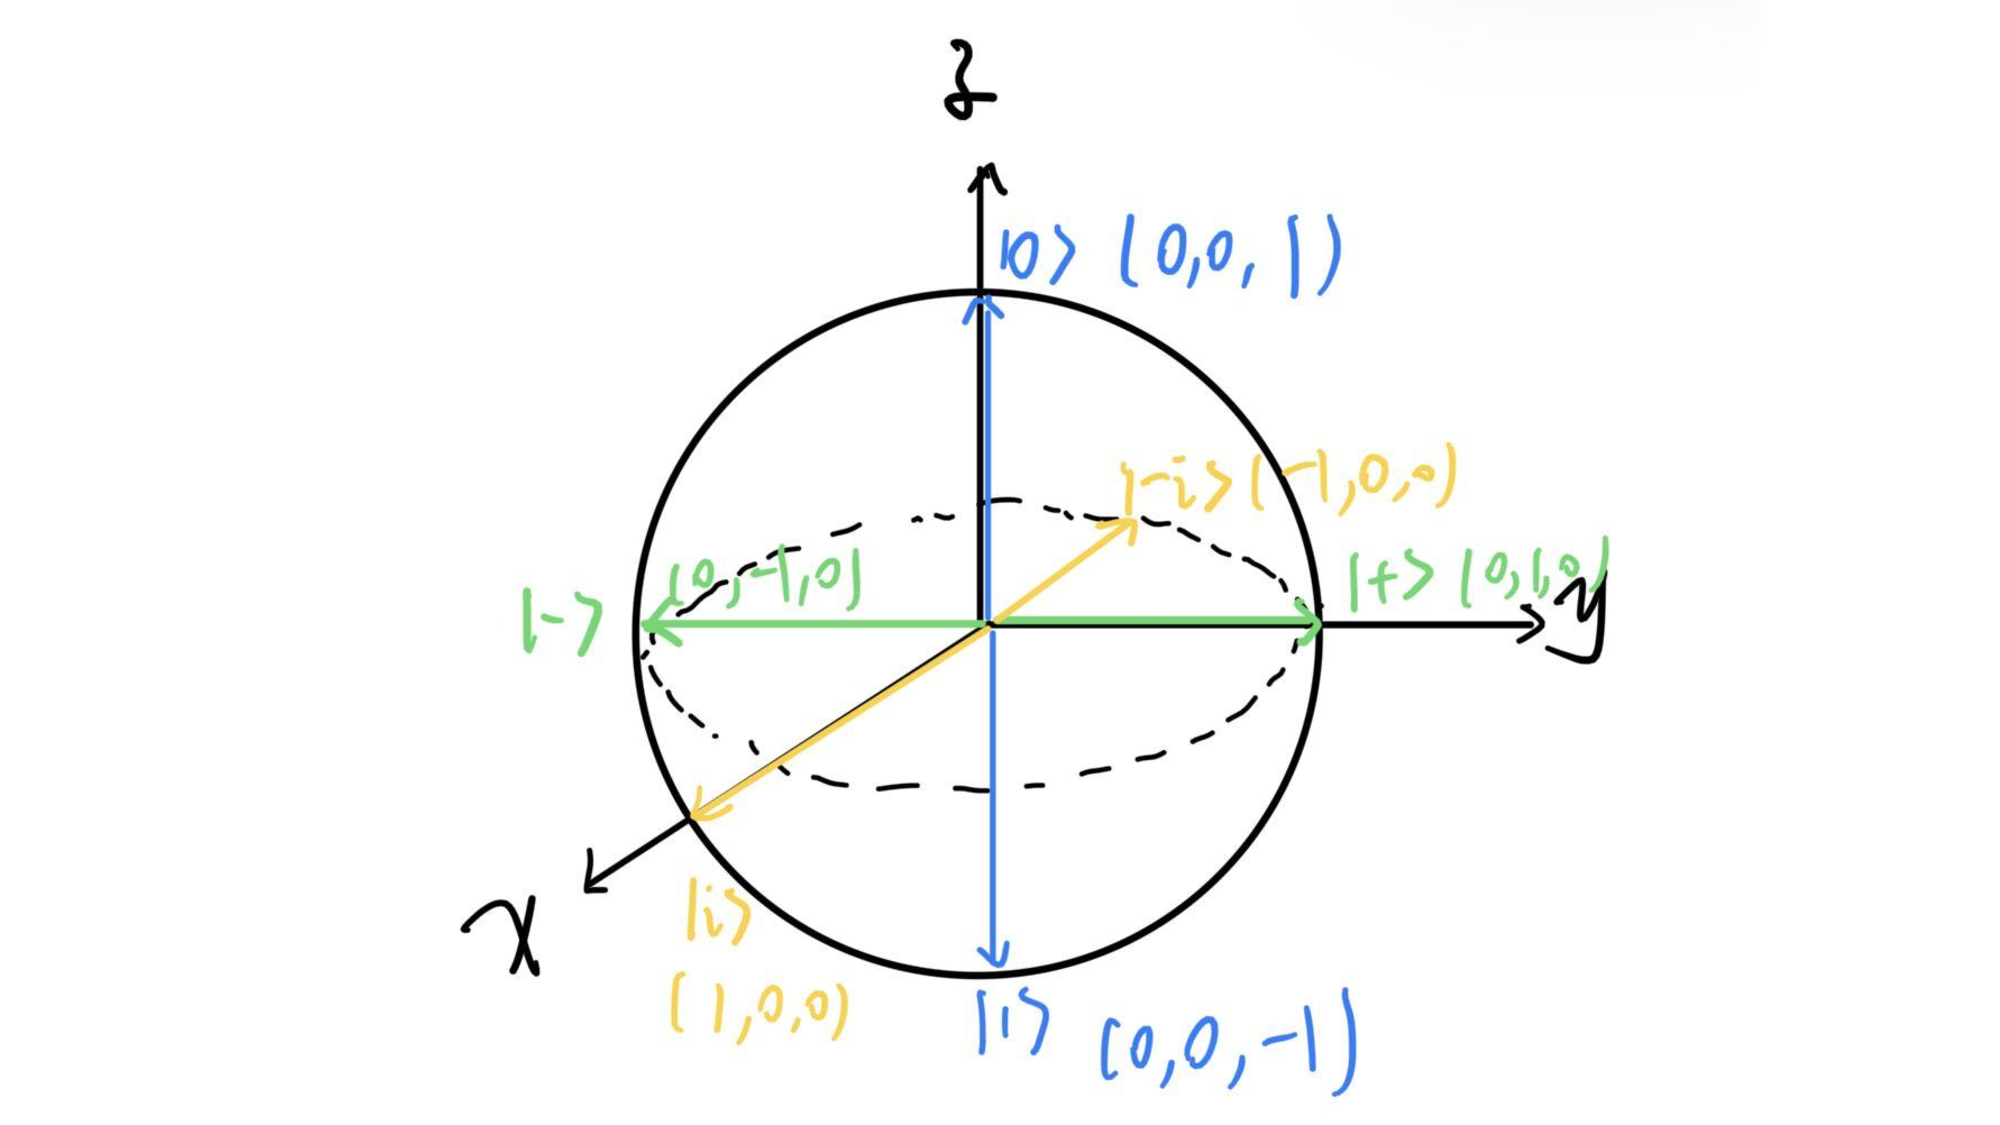
\includegraphics[height=5cm]{BS.pdf}
          \end{figure}
          $\frac{I}{2}=
              \left(
              \begin{array}{cc}
                      \frac{1}{2} & 0 \\0&\frac{1}{2}
                  \end{array}
              \right)
              =\frac{1}{2}\left(
              \begin{array}{cc}
                      1 & 0 \\0&1\\
                  \end{array}
              \right)
              =\frac{1}{2}(I+O)
          $

          So, $\vec{r}\vec{\sigma}=O$

          Assume $\vec{r}=(a,b,c)^T$

          $\vec{r}\vec{\sigma}
              \\=(a,b,c)^T(\left(
              \begin{array}{cc}
                      0 & 1 \\1&0\\
                  \end{array}
              \right)\left(
              \begin{array}{cc}
                      0 & -i \\i&0\\
                  \end{array}
              \right)\left(
              \begin{array}{cc}
                      1 & 0 \\0&-1\\
                  \end{array}
              \right))
              \\=\left(
              \begin{array}{cc}
                      0 & a \\a&0\\
                  \end{array}
              \right)+\left(
              \begin{array}{cc}
                      0 & -bi \\bi&0\\
                  \end{array}
              \right)+\left(
              \begin{array}{cc}
                      c & 0 \\0&-c\\
                  \end{array}
              \right)
              \\=\left(
              \begin{array}{cc}
                      c & a-bi \\a+bi&-c\\
                  \end{array}
              \right)
          $

          So, $\left(
              \begin{array}{cc}
                      c & a-bi \\a+bi&-c\\
                  \end{array}
              \right)=O=\left(
              \begin{array}{cc}
                      0 & 0 \\0&0\\
                  \end{array}
              \right)$

          which means $a=b=c=0$ and $\vec{r}=(0,0,0)^T$

          So, $\frac{I}{2}$ is located in $(0,0,0)$, which is the centre of the Bloch ball.
    \item \begin{enumerate}
              \item $\rho_1
                        \\=\frac{1}{2}(I+\vec{r}\vec{\sigma})
                        \\=\frac{1}{2}(I+(0,-\frac{1}{3},0)\vec{\sigma})
                        \\=\frac{1}{2}(I+\left(
                        \begin{array}{cc}
                                0 & \frac{1}{3}i \\-\frac{1}{3}i&0\\
                            \end{array}
                        \right))
                        \\==\frac{1}{2}(\left(
                        \begin{array}{cc}
                                1 & \frac{1}{3}i \\-\frac{1}{3}i&1\\
                            \end{array}
                        \right))
                        \\=(\left(
                        \begin{array}{cc}
                                \frac{1}{2} & \frac{1}{6}i \\-\frac{1}{6}i&\frac{1}{2}\\
                            \end{array}
                        \right))
                    $

                    Because $\rho_1^2=\left(
                        \begin{array}{cc}
                                \frac{1}{2} & \frac{1}{6}i \\-\frac{1}{6}i&\frac{1}{2}\\
                            \end{array}
                        \right)\left(
                        \begin{array}{cc}
                                \frac{1}{2} & \frac{1}{6}i \\-\frac{1}{6}i&\frac{1}{2}\\
                            \end{array}
                        \right)=\left(
                        \begin{array}{cc}
                                \frac{11}{36} & 0 \\0&\frac{11}{36}\\
                            \end{array}
                        \right)
                    $,

                    $Tr(\rho_1^2)=\frac{11}{18}\neq1$,
                    $\rho_1$ is nota pure state.
              \item $\rho_2
                        \\=\frac{1}{2}(I+\vec{r}\vec{\sigma})
                        \\=\frac{1}{2}(I+(-\frac{1}{2},\frac{1}{2},0)\vec{\sigma})
                        \\=\frac{1}{2}(I+\left(
                        \begin{array}{cc}
                                0 & \frac{-1-i}{\sqrt{2}}i \\-\frac{-1+i}{\sqrt{2}}i&0\\
                            \end{array}
                        \right))
                        \\==\frac{1}{2}(\left(
                        \begin{array}{cc}
                                1 & \frac{-1-i}{\sqrt{2}}i \\\frac{-1+i}{\sqrt{2}}i&1\\
                            \end{array}
                        \right))
                        \\=(\left(
                        \begin{array}{cc}
                                \frac{1}{2} & \frac{-1-i}{2\sqrt{2}}i \\\frac{-1+i}{2\sqrt{2}}i&\frac{1}{2}\\
                            \end{array}
                        \right))
                    $



                    $\rho_2^2=\left(
                        \begin{array}{cc}
                                \frac{1}{2} & \frac{-1-i}{2\sqrt{2}}i \\\frac{-1+i}{2\sqrt{2}}i&\frac{1}{2}\\
                            \end{array}
                        \right)\left(
                        \begin{array}{cc}
                                \frac{1}{2} & \frac{-1-i}{2\sqrt{2}}i \\\frac{-1+i}{2\sqrt{2}}i&\frac{1}{2}\\
                            \end{array}
                        \right)=\left(
                        \begin{array}{cc}
                                \frac{1}{2} & \frac{-1-i}{2\sqrt{2}}i \\\frac{-1+i}{2\sqrt{2}}i&\frac{1}{2}\\
                            \end{array}
                        \right)
                        =\rho_2
                    $,

                    Because $Tr(\rho_2^2)=1$, $\rho_2$ is nota pure state.
          \end{enumerate}
    \item The surface of the Bloch sphere.

          \textbf{PROOF:}

          Assume a pure state $\ket{\psi}$'s Bloch vector $\vec{r}=(a,b,c)^T$.

          $\rho=\frac{1}{2}(I+\vec{r}\vec{\sigma})
              \\=\frac{1}{2}(I+\left(
              \begin{array}{cc}
                      c & a-bi \\a+bi&-c\\
                  \end{array}
              \right))
              \\=\frac{1}{2}\left(
              \begin{array}{cc}
                      1+c & a-bi \\a+bi&1-c\\
                  \end{array}
              \right)
              \\=\left(
              \begin{array}{cc}
                      \frac{1+c}{2} & \frac{a-bi}{2} \\\frac{a+bi}{2}&\frac{1-c}{2}\\
                  \end{array}
              \right)
          $

          $\rho^2=\left(
              \begin{array}{cc}
                      \frac{1+c}{2} & \frac{a-bi}{2} \\\frac{a+bi}{2}&\frac{1-c}{2}\\
                  \end{array}
              \right)\left(
              \begin{array}{cc}
                      \frac{1+c}{2} & \frac{a-bi}{2} \\\frac{a+bi}{2}&\frac{1-c}{2}\\
                  \end{array}
              \right)
              \\=\left(
              \begin{array}{cc}
                      \frac{(1+c)^2+a^2-(bi)^2}{4} & \frac{(1+c)(a-bi)+(a-bi)(1-c)}{4} \\\frac{(a+bi)(1+c)+(1-c)(a+bi)}{4}&\frac{a^2-(bi)^2+(1-c)^2}{4}\\
                  \end{array}
              \right)
          $

          $Tr(\rho^2)
              \\=\frac{(1+c)^2+a^2-(bi)^2}{4}+\frac{a^2-(bi)^2+(1-c)^2}{4}
              \\=\frac{(1+c)^2+a^2-(bi)^2+a^2-(bi)^2+(1-c)^2}{4}
              \\=\frac{2a^2+2b^2+c^2+2c+1+c^2-2c+1}{4}
              \\=\frac{2(a^2+b^2+c^2)+2}{4}
          $

          Because $\ket{\psi}$ is a pure state, so $Tr(\rho^2)$=1, which means $\frac{2(a^2+b^2+c^2)+2}{4}=1$.

          So, $a^2+b^2+c^2=1$, this means $\vec{r}=(a,b,c)^T$ is on the surface of the Bloch sphere, pure state $\ket{\psi}$ is on the surface of the Bloch sphere.



    \item The requirements of sensity matracies are as followed,
          \begin{enumerate}
              \item \textbf{Positive semi-definite:} all eigenvalues $\lambda_i\geq0$
              \item \textbf{Hermitian:} $\rho=\rho^{\dag}$
              \item \textbf{Normalization:} $Tr(\rho)=1$
          \end{enumerate}


          For vector $\vec{r}$, $\rho=\frac{1}{2}(I+\vec{r}\vec{\sigma})=\left(
              \begin{array}{cc}
                      \frac{1+c}{2} & \frac{a-bi}{2} \\\frac{a+bi}{2}&\frac{1-c}{2}\\
                  \end{array}
              \right)$

          Assume the eigenvalues of $\rho$ are $\lambda_1,...,\lambda_n$

          $\left|
              \left(
              \begin{array}{cc}
                      \frac{1+c}{2} & \frac{a-bi}{2} \\\frac{a+bi}{2}&\frac{1-c}{2}\\
                  \end{array}
              \right)-\lambda I\right|=0$

          $\left|
              \begin{array}{cc}
                  \frac{1+c}{2}-\lambda & \frac{a-bi}{2} \\\frac{a+bi}{2}&\frac{1-c}{2}-\lambda\\
              \end{array}
              \right|=0$

          $(\frac{1+c}{2}-\lambda )(\frac{1-c}{2}-\lambda)-(\frac{a-bi}{2})(\frac{a+bi}{2})=0$

          $\frac{1-c^2}{4}-(\frac{1+c+1-c}{2}\lambda)+\lambda^2-\frac{a^2+b^2}{4}=0$

          $\lambda^2-\lambda+\frac{1-a^2-b^2-c^2}{4}=0$

          $\lambda=\frac{1\pm \sqrt{1-4\times\frac{1-a^2-b^2-c^2}{4}}}{2}=\frac{1\pm\sqrt{a^2+b^2+c^2}}{2}=\frac{1\pm\sqrt{|\vec{r}|^2}}{2}$

          Because $|\vec{r}|\leq1$, $\frac{1\pm\sqrt{|\vec{r}|^2}}{2} \in [0,1]$, which means $0\leq\lambda\leq1$, this proves the \textbf{Positive semi-definite}.

          $\rho^{\dag}=
              \left(
              \begin{array}{cc}
                      \frac{1+c}{2} & (\frac{a+bi}{2})^* \\(\frac{a-bi}{2})^*&\frac{1-c}{2}\\
                  \end{array}
              \right)
              =\left(
              \begin{array}{cc}
                      \frac{1+c}{2} & \frac{a-bi}{2} \\\frac{a+bi}{2}&\frac{1-c}{2}\\
                  \end{array}
              \right)=\rho$

          This proves the \textbf{Hermitian}.

          The trace of matrix $\rho$

          $Tr(\rho)=\lambda_1+\lambda_2=\frac{1+\sqrt{|\vec{r}|^2}}{2}+\frac{1-\sqrt{|\vec{r}|^2}}{2}=1$.

          This proves the \textbf{Normalization}.



          So $\rho$ is indeed a valid density operator for any vector $\vec{r}$ satisfing $|\vec{r}|\leq1$.
\end{enumerate}
\begin{thebibliography}{1}
    \bibitem{ref1}HKUST Department of Mathematics.
    "Inner Product Spaces and Orthogonality"
    Hong Kong University of Science and Technology, n.d.,
    https://www.math.hkust.edu.hk/~mabfchen/Math111/Week13-14.pdf.
\end{thebibliography}
\end{document}